


\documentclass[a4paper]{article}

\usepackage[utf8]{inputenc}
\usepackage[french]{babel}
\usepackage{graphicx}
\graphicspath{{./img/}}
\usepackage{amsmath, amssymb}
\usepackage[left=3cm,right=3cm,top=2cm,bottom=2cm]{geometry}
\usepackage{url}
\usepackage{listings}


\usepackage[french]{babel}
\title{TP n°1 : Entropies discrète et continue, information mutuelle}
\author{Aarab Wassim - Dlimi Mohammed - Ettaki Mohammed Amine}
\date{Décembre 2023}



\begin{document}
\maketitle
\tableofcontents
\newpage
%exo 1 :
\section{Lien entre entropie discrète et continue}
$X$ est une variable aléatoire de densité $f_{X}$ continue.\\
$\forall \Delta > 0$, $X_{\Delta} = \sum_{i\in \mathbb{Z}} x_{i}\mathbb{1}_{[i\Delta,(i+1)\Delta]}(X)$ où $x_i \in [i\Delta,(i+1)\Delta]$.\\

\[
1- \quad
\frac{1}{\Delta} \int_{i\Delta}^{(i+1)\Delta} f_X(x) \, dx = \frac{1}{\Delta} (F_X((i+1)\Delta) - F_X(i\Delta)) = \frac{F_X((i+1)\Delta) - F_X(i\Delta)}{(i+1)\Delta - i\Delta}
\]

D'après le théorème des accroissements finis appliqués sur $F_X$ sur $[i\Delta,(i+1)\Delta]$: \\
\[
\forall i \in \mathbb{Z}, \exists x_i \in ]i\Delta,(i+1)\Delta[, \quad f_X(x_i) = \frac{1}{\Delta} \int_{i\Delta}^{(i+1)\Delta} f_X(x) \,dx
\]

\[
2- \quad
P(X_\Delta = x_i) = P(i\Delta \leq X \leq (i+1)\Delta) = \int_{i\Delta}^{(i+1)\Delta} f_X(x) \, dx = \Delta f_X(x_i) 
\]

\begin{align*}
    3- \quad H(X_\Delta) & = E(-\log(P_X\Delta)) \\
    & = \sum_{i\in \mathbb{Z}} -P(X_\Delta=x_i)\log(P(X_\Delta = x_i)) \\
    & = - \sum_{i\in \mathbb{Z}} \Delta f_X(x_i)\log(\Delta f_X(x_i)) \\
    & = - \Delta\left(\sum_{i\in \mathbb{Z}} f_X(x_i)\log(f_X(x_i)) + \log(\Delta) \sum_{i\in \mathbb{Z}} f_X(x_i)\right) \\
    & = - \Delta\sum_{i\in \mathbb{Z}} f_X(x_i)\log(f_X(x_i)) - \log(\Delta)
\end{align*}


\newpage

%exo 2 Partie 1:
\section{Loi gaussienne}
\subsection{Loi gaussienne univariée.}
on considère maintenant une variable aléatoire réelle $X$ qui suit une loi gaussienne de moyenne $\mu$ et de variance $\sigma^{2}$ (ie. $X \sim \mathcal{N}(\mu, \sigma^{2}))$, on veut maintenant vérifier numériquement le résultat théorique obtenu précédemment pour une variable qui suit une loi gaussienne. Il suffit donc de considérer un nombre très grand de réalisations différentes de $X$ notées $x_i$ pour qu'on puisse définir $X_{\Delta}$ avec un $\Delta$ très petit, car plus le nombre des $x_i$ qu'on choisit est grand plus que la distance entre ses éléments qui est égale à $\Delta$ est petite. On choisit par exemple $n=10000$ réalisations.\\
Pour vérifier maintenant numériquement que la densité de cette loi est bien $f_{X}=\frac{1}{\sigma\sqrt{2\pi}}\exp\left(-\frac{(x-\mu)^{2}}{2\sigma^2}\right)$, on trace l'histogramme de ces $n$ réalisations $x_{i}$ d'une aire normalisée à 1 et la densité $f_{X}$ dans une même figure. On trouve la figure ci-dessous.

\begin{figure}[h]
  \centering
  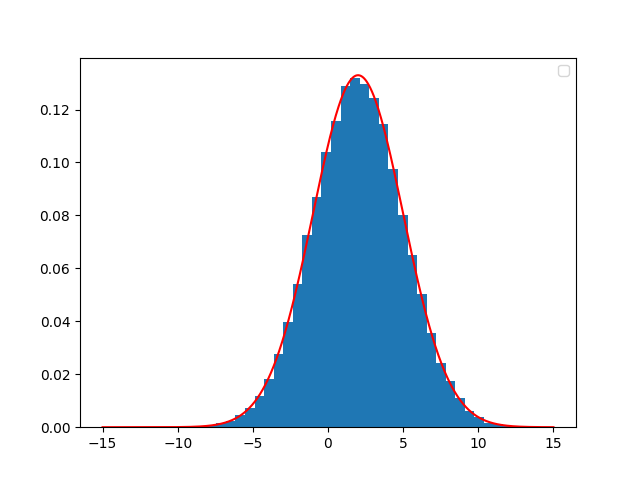
\includegraphics[width=0.8\textwidth]{Figure_1.png}
  \caption{histogramme-densité}
%  \label{hist}
\end{figure}
ceci prouve que la densité de $X$ est bien $f_X$ puisque les deux graphes sont compatibles,il nous reste maintenant à vérifier le résultat$\mathbb{H}(X_\Delta)+\log(\Delta)\underset{\Delta \rightarrow 0}{\rightarrow}\mathbb{H}(X)$,pour se faire,on calcule tout d'abord le membre gauche de la relation à l'aide d'un code python avec $\Delta=1/n$ qui tend vers 0 fourni en annexe,et en testant on trouve la valeur $0.21314555932018384$,ensuite en calcule théoriquement $\mathbb{H}(X)$ comme ci dessous:
\begin{align*}
  \mathbb{H}(X) &= -\int_{-\infty}^{\infty}f_{X}\log(f_X(x))\,dx \\
  &= -\int_{-\infty}^{\infty}\frac{1}{\sigma\sqrt{2\pi}}\exp\left(-\frac{(x-\mu)^{2}}{2\sigma^2}\right)\log\left(\frac{1}{\sigma\sqrt{2\pi}}\exp\left(-\frac{(x-\mu)^{2}}{2\sigma^2}\right)\right)\,dx \\
  &= \int_{-\infty}^{\infty}\left(\frac{\log(3\sqrt{2\pi})}{3\sqrt{2\pi}}\exp\left(-\frac{(x-2)^2}{18}\right) + \frac{1}{3\sqrt{2\pi}}\left(\frac{(x-2)^2}{18}\right)\exp\left(-\frac{(x-2)^2}{18}\right)\right)\,dx
\end{align*}
et on a d'après les intégrales de Gauss : $\int_{-\infty}^{\infty}\exp{-x^2}=\sqrt{\pi}$ et $\int_{\infty}^{\infty}x^2\exp(-x^2)=\frac{\sqrt{\pi}}{2}$ et donc par conséquent : 
\begin{align*}
  \mathbb{H}(X) &= \frac{1}{2}+\log(3\sqrt{2\pi})\\
  \mathbb{H}(X) &= 2.51755
\end{align*}
cette valeur est très loin de la valeur obtenue numériquement,la relation n'est pas donc satisfaite pour une loi gaussièene univariée


\newpage

%exo 2 Partie 2:
\subsection{Loi gaussienne multivariée.}
Soit \(\mu \in \mathbb{R}^p\) et \(X \in \mathcal{M}_p(\mathbb{R})\), pour générer des réalisations de \(X\), le processus se déroule en deux étapes :

1. Dans la première étape, la fonction \texttt{np.random.randn} est utilisée pour créer une matrice \(Z\) où chaque ligne représente un échantillon indépendant d'une loi normale univariée \(N(0,1)\).

\[
Z = \begin{bmatrix}
    Z_{1,1} & Z_{1,2} & \ldots & Z_{1,p} \\
    Z_{2,1} & Z_{2,2} & \ldots & Z_{2,p} \\
    \vdots  & \vdots  & \ddots & \vdots  \\
    Z_{n,1} & Z_{n,2} & \ldots & Z_{n,p}
\end{bmatrix}
\]

2. Dans la deuxième étape, une transformation linéaire est appliquée à ces échantillons en utilisant la décomposition de Cholesky de la matrice de covariance \(R\). Cela donne des échantillons de la loi normale multivariée recherchée \(X = \mu + Z \cdot L^T\), où \(Z\) est la matrice des échantillons de la loi normale univariée et \(L\) est la matrice triangulaire inférieure de la décomposition de Cholesky de \(R\).
on essaie maintenant d'appliquer ça dans un programme python comme celui fourni en annexe C,on obtient les résultats suivantes :
\begin{figure}[h]
  \centering
  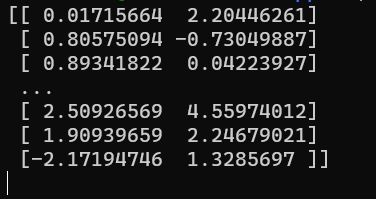
\includegraphics[width=0.7\textwidth]{6.png}
  \caption{expemple de réalisations}
%  \label{hist}
\end{figure}
on superpose maintenant,à l'aide d'un code python fourni dans l'annexe D,dans une meme figure les lignes de niveaux de la densité de la loi gaussienne unvarié et l'histogramme de X on trouve la figure suivant
\begin{figure}[h]
  \centering
  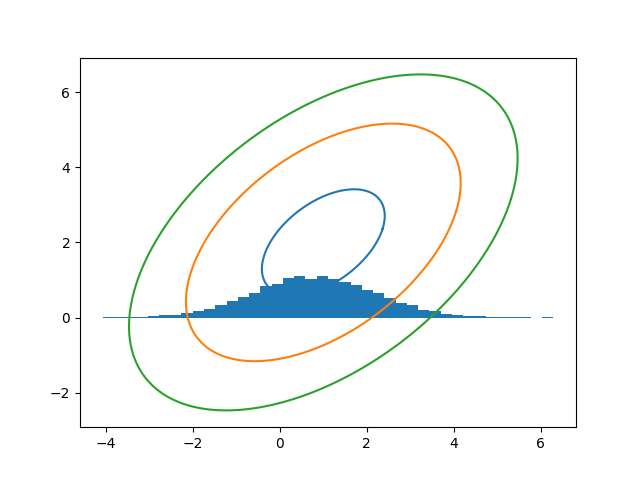
\includegraphics[width=0.7\textwidth]{7.png}
  \caption{niveaux densité}
%  \label{hist}
\end{figure}
on constate donc trois ellipses parallèles.
%exo3 : 
\section{Analyse de données}
\newpage
\appendix
\section{Annexe A}
\begin{figure}[h]
  \centering
  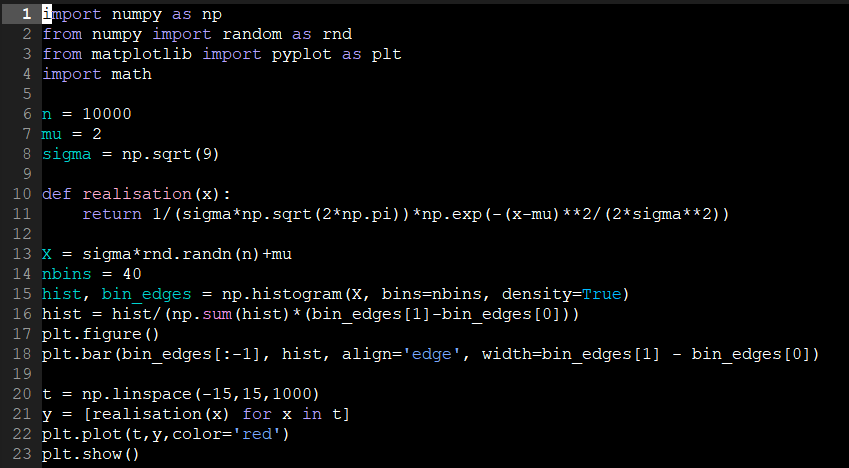
\includegraphics[width=0.8\textwidth]{1.png}
  \caption{python histogramme-densité}
%  \label{hist}
\end{figure}

\section{Annexe B}
\begin{figure}[h]
  \centering
  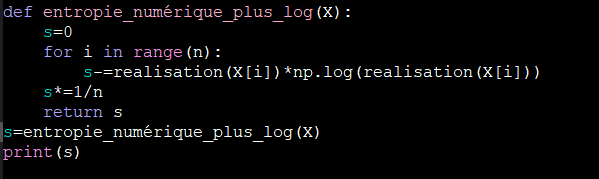
\includegraphics[width=0.8\textwidth]{4.png}
  \caption{entropie numérique}
%  \label{hist}
\end{figure}
\section{Annexe C}
\begin{figure}[h]
  \centering
  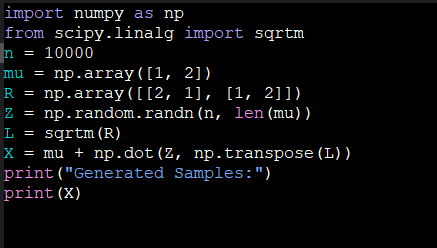
\includegraphics[width=0.5\textwidth]{5.png}
  \caption{réalisations d'un vectur}
%  \label{hist}
\end{figure}
\newpage
\section{Annexe D}
\begin{figure}[h]
  \centering
  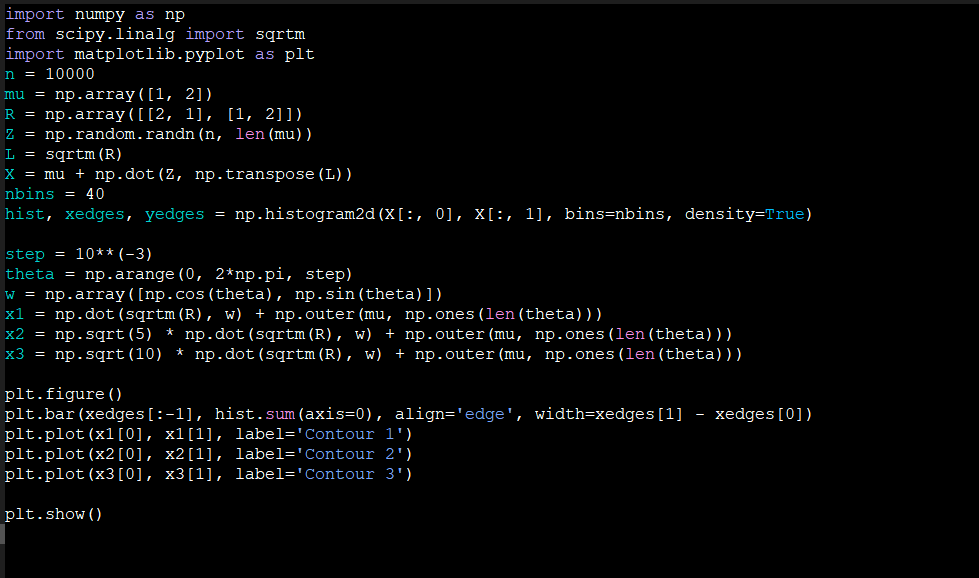
\includegraphics[width=0.5\textwidth]{8.png}
  \caption{code niveaux densité}
%  \label{hist}
\end{figure}



\end{document}
